%%%%%%%%%%%%%%%%%%%%%%%%%%%%%%%%%%%%%%%%%
% Wenneker Assignment
% LaTeX Template
% Version 2.0 (12/1/2019)
%
% This template originates from:
% http://www.LaTeXTemplates.com
%
% Authors:
% Vel (vel@LaTeXTemplates.com)
% Frits Wenneker
%
% License:
% CC BY-NC-SA 3.0 (http://creativecommons.org/licenses/by-nc-sa/3.0/)
% 
%%%%%%%%%%%%%%%%%%%%%%%%%%%%%%%%%%%%%%%%%

%----------------------------------------------------------------------------------------
%	PACKAGES AND OTHER DOCUMENT CONFIGURATIONS
%----------------------------------------------------------------------------------------

\documentclass[11pt]{scrartcl} % Font size

%%%%%%%%%%%%%%%%%%%%%%%%%%%%%%%%%%%%%%%
% Wenneker Assignment
% Structure Specification File
% Version 2.0 (12/1/2019)
%
% This template originates from:
% http://www.LaTeXTemplates.com
%
% Authors:
% Vel (vel@LaTeXTemplates.com)
% Frits Wenneker
%
% License:
% CC BY-NC-SA 3.0 (http://creativecommons.org/licenses/by-nc-sa/3.0/)
% 
%%%%%%%%%%%%%%%%%%%%%%%%%%%%%%%%%%%%%%%%%

%----------------------------------------------------------------------------------------
%	PACKAGES AND OTHER DOCUMENT CONFIGURATIONS
%----------------------------------------------------------------------------------------
\usepackage{xcolor}   % for \textcolor
\usepackage{comment}

\usepackage{amsmath, amsfonts, amsthm} % Math packages

\usepackage{listings} % Code listings, with syntax highlighting
\usepackage{verbatim} % Directly from txt file

\usepackage[english]{babel} % English language hyphenation
\usepackage{tikz} 
\usepackage{neuralnetwork} 
\usepackage{graphicx} % Required for inserting images
\graphicspath{{Figures/}{./}} % Specifies where to look for included images (trailing slash required)
\usepackage{setspace}  % allows linespacing changes
\usepackage{tabularx} % for tables

\usepackage{booktabs} % Required for better horizontal rules in tables

\numberwithin{equation}{section} % Number equations within sections (i.e. 1.1, 1.2, 2.1, 2.2 instead of 1, 2, 3, 4)
\numberwithin{figure}{section} % Number figures within sections (i.e. 1.1, 1.2, 2.1, 2.2 instead of 1, 2, 3, 4)
\numberwithin{table}{section} % Number tables within sections (i.e. 1.1, 1.2, 2.1, 2.2 instead of 1, 2, 3, 4)

\setlength\parindent{0pt} % Removes all indentation from paragraphs

\usepackage{enumitem} % Required for list customisation
\setlist{noitemsep} % No spacing between list items

%----------------------------------------------------------------------------------------
%	DOCUMENT MARGINS
%----------------------------------------------------------------------------------------

\usepackage{geometry} % Required for adjusting page dimensions and margins

\geometry{
	paper=a4paper, % Paper size, change to letterpaper for US letter size
	top=2.5cm, % Top margin
	bottom=3cm, % Bottom margin
	left=3cm, % Left margin
	right=3cm, % Right margin
	headheight=0.75cm, % Header height
	footskip=1.5cm, % Space from the bottom margin to the baseline of the footer
	headsep=0.75cm, % Space from the top margin to the baseline of the header
	%showframe, % Uncomment to show how the type block is set on the page
}

%----------------------------------------------------------------------------------------
%	FONTS
%----------------------------------------------------------------------------------------

\usepackage[utf8]{inputenc} % Required for inputting international characters
\usepackage[T1]{fontenc} % Use 8-bit encoding

\usepackage{fourier} % Use the Adobe Utopia font for the document

%----------------------------------------------------------------------------------------
%	SECTION TITLES
%----------------------------------------------------------------------------------------

\usepackage{sectsty} % Allows customising section commands

\sectionfont{\vspace{6pt}\centering\normalfont\scshape} % \section{} styling
\subsectionfont{\normalfont\bfseries} % \subsection{} styling
\subsubsectionfont{\normalfont\itshape} % \subsubsection{} styling
\paragraphfont{\normalfont\scshape} % \paragraph{} styling

%----------------------------------------------------------------------------------------
%	HEADERS AND FOOTERS
%----------------------------------------------------------------------------------------

\usepackage{scrlayer-scrpage} % Required for customising headers and footers

\ohead*{} % Right header
\ihead*{} % Left header
\chead*{} % Centre header

\ofoot*{} % Right footer
\ifoot*{} % Left footer
\cfoot*{\pagemark} % Centre footer
 % Include the file specifying the document structure and custom commands
\usepackage{cite}

\usepackage{hyperref}

%----------------------------------------------------------------------------------------
%	TITLE SECTION
%----------------------------------------------------------------------------------------

\title{	
	\normalfont\normalsize
	\textsc{Intelligent Robotics, Portland State University}\\ % Your university, school and/or department name(s)
	\vspace{25pt} % Whitespace
	\rule{\linewidth}{0.5pt}\\ % Thin top horizontal rule
	\vspace{20pt} % Whitespace
	{\huge Winter Report}\\ % The assignment title
	\vspace{4pt} % Whitespace
	{\large Quaternion Attitude Control of a Simulated Airplane}\\ % The assignment title
	\vspace{12pt} % Whitespace
	\rule{\linewidth}{2pt}\\ % Thick bottom horizontal rule
	\vspace{12pt} % Whitespace
}

\author{\LARGE Trenton Ruf} % Your name
\date{\normalsize \today} % Today's date (\today) or a custom date

\begin{document}
\maketitle % Print the title
%\renewcommand\thesubsection{\Alph{subsection}}
%\renewcommand\thesubsection{\Roman{subsection}}
%\doublespacing
%\singlespace
%\onehalfspacing
%\setstretch{1.25}

%\begin{doublespace}
%\end{doublespace}

%\vspace*{\fill}
%\clearpage
%\vspace*{\fill}


%\vspace*{\fill}
\renewcommand\thesubsection{\Roman{subsection}}
%\section{Loading Pre-Trained Model}
\section{Changes to Last Term's code}
I made the fuzzy-altitude controller from last term into a ROS service server. This is to control the attitude setpoint and enable/disable the controller from a seperate ROS node. My plan is to have the altitude and attitude controller nodes given commands by a master "State Machine" node.


\section{Quaternion Control}
\subsection{Layout}
The quaternion attitude controller was modeled after \underline{Quaternion Attitude Control System of Highly Maneuverable Aircraft} ~\cite{quat}.
It is a cascading controller that takes a quaternion setpoint ($q_{sp}$) as the initial intput

\begin{figure}[ht!] % [h] forces the figure to be output where it is defined in the code (it suppresses floating)
	\centering
	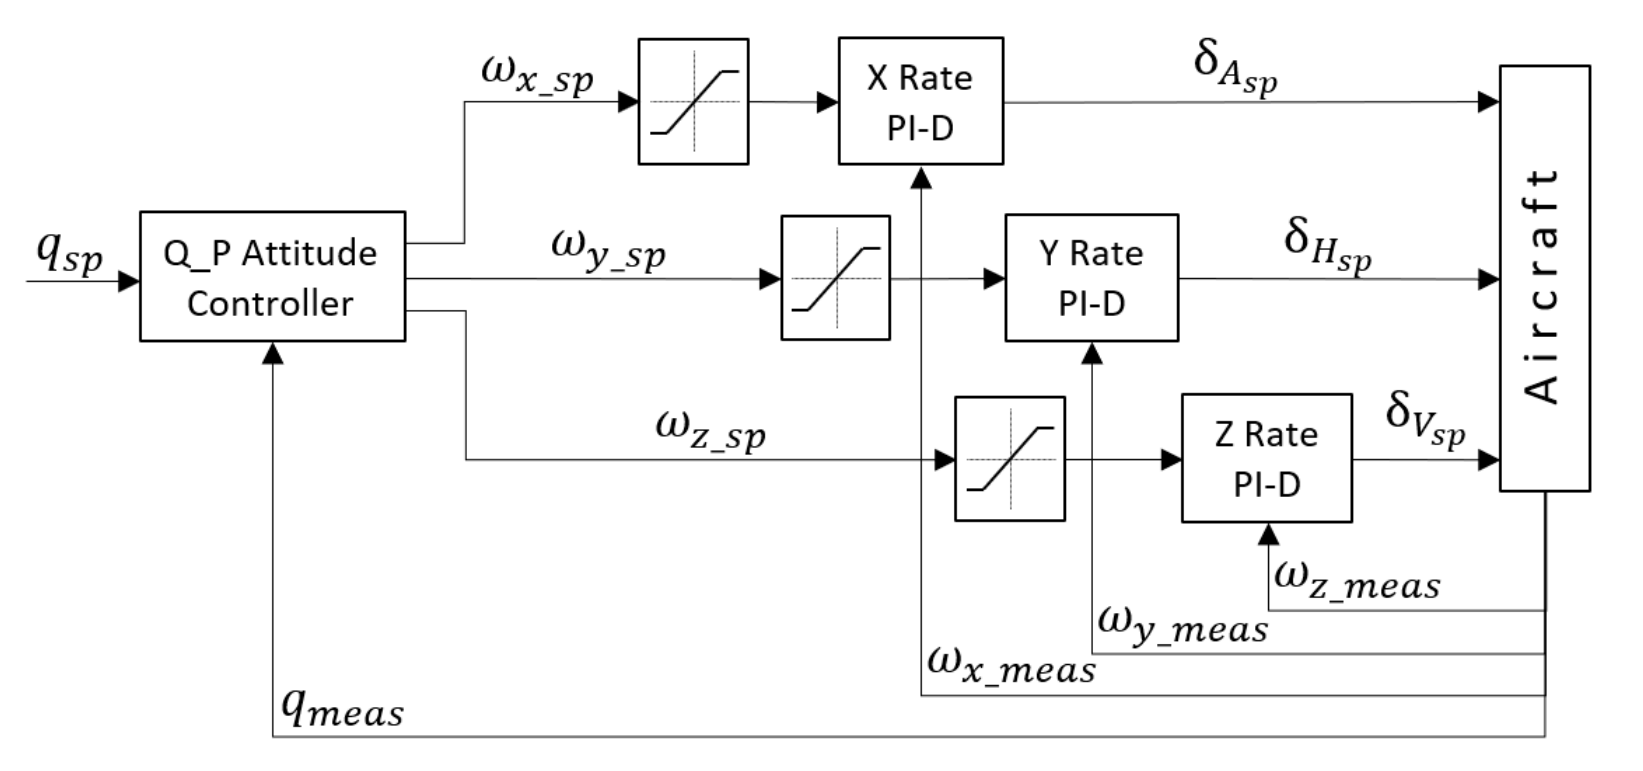
\includegraphics[width=0.9\columnwidth]{QuatSchematicPID.png} 
	\caption{Quaternion-Based controller schematic from ~\cite{quat}}
\end{figure}



\subsection{Roslaunch}
I followed the guides on the official ROSflight website cover the installation of ROS, ROSflight, and the Gazebo simulator. I modified the default Roslaunch file for simulating a fixed-wing aircraft to include rosflight\_joy, a companion node that binds keystrokes to a simulated Radio Controller to manually maneuver the aircraft. The RC controller is necessary to "arm" the plane before the throttle can be activated. Since ROSflight is designed to run on an actual aircraft, there is a bit of configuration required begin simulations. You must calibrate the IMU and set the appropriate fixed wing parameters (i.e. tell ROSflight it is a plane and not a multi-copter). More details can be found in the official documentation. The modified roslaunch file called myfixedwing.launch includes links to two separate world files I created. Both of these worlds are airfields but unfortunately the computer I am running the simulation on currently cannot render them in real-time, so they are currently disabled.

\subsection{Gazebo}
The Gazebo installation should happen along side ROSflight, but you may encounter the following error when first running a simulation: 

\small
\color{red}
[Err] [ModelDatabase.cc:235] No <database> tag in the model database database.config found here[\url{http://gazebosim.org/models/}]

[Err] [ModelDatabase.cc:294] Unable to download model manifests
\\
\color{black}
\normalsize

The location of the model database has changed but has not been reflected in the gazebo package yet. The fix is to redirect to the correct URL before running the any launch files:

\small
\color{green}
export GAZEBO\_MODEL\_DATABASE\_URI=\url{http://models.gazebosim.org/}
\\ \color{black}
\normalsize

The gazebo website is undergoing a major reconstruction at the moment. You should open up the URL above in a web browser too to check if the fix is still working.




\section{altitude hold pid}
The ROSflight node outputs a "Barometer" message that contains temperature, pressure, and altitude data. It also listens on the "Command" message for setting the plane's throttle, aileron, elevator, and rudder control surface positions. I created a new node called altitudePID that subscribes to the altitude reading and publishes an elevator position command. The mapping of altitude inputs to elevator outputs was done with a PID controller from the "simple\_pid" python library. The tuning of the PID gains was conducted with a trial and error approach. I followed the Ziegler–Nichols method for the most part. The altitude hold setpoint was hard-coded to be 10 Meters above the ground. All control surfaces have a deflection range of (-1,1). That said during normal flight they should never get close to the maximum ranges. When testing full elevator deflection in flight the plane immediately turns 90 degrees and stalls.

\section{fuzzy pid!}
The altitudePID node works well for holding altitude while the wings are level, but an abrupt bank will begin large altitude oscillations. I believe this is due to the amount vertical lift that the elevator can influence being decreased with larger bank angles. The PID controller was tuned for maximum lift influence, so it makes sense that it will have problems when it falls out its ideal environment. To fix this issue the gains of the PID controller need to be altered during operation.  
\\

I found a white paper that covers an implementation of fuzzy-inference for airplane pitch control~\cite{fuzzy}. Since pitch is controlled with the elevator position I believed it would also work as an altitude controller. I created the "fuzzy-altitudePID" node that takes the fuzzy logic rules presented in the paper and integrates them with the altitudePID node from earlier. While the rules where kept the same I changed the ranges of all other parameters. All of these values where found from experimentation. For instance, the error delta range was determined by sending large manual inputs to the plane in flight to see what maximum and minimum error values could be. The tuning method from the original altitudePID node did not work for the fuzzy rule set. 

\subsection{code}

All files related to this project can be found at:

\url{https://github.com/Trenton-Ruf/Intelligent_Robotics}

\lstinputlisting[
	caption= altitudePID, % Caption above the listing
	%label=lst:test, % Label for referencing this listing
	language=Python, % Use Perl functions/syntax highlighting
	frame=single, % Frame around the code listing
	breaklines=true,
	postbreak=\mbox{\textcolor{red}{$\hookrightarrow$}\space},	
	showstringspaces=false, % Don't put marks in string spaces
	numbers=left, % Line numbers on left
	numberstyle=\tiny, % Line numbers styling
	basicstyle=\footnotesize
	]{../../../catkin_ws/src/rosflight_control/src/altitudePID.py}

\lstinputlisting[
	caption= fuzzy-altitudePID, % Caption above the listing
	%label=lst:test, % Label for referencing this listing
	language=Python, % Use Perl functions/syntax highlighting
	frame=single, % Frame around the code listing
	breaklines=true,
	postbreak=\mbox{\textcolor{red}{$\hookrightarrow$}\space},	
	showstringspaces=false, % Don't put marks in string spaces
	numbers=left, % Line numbers on left
	numberstyle=\tiny, % Line numbers styling
	basicstyle=\footnotesize
	]{../../../catkin_ws/src/rosflight_control/src/fuzzy-altitudePID.py}


\clearpage
\medskip

\bibliography{resources.bib}{}
\bibliographystyle{IEEEtran}

\end{document}
